\documentclass[12pt]{article}

\usepackage[utf8]{inputenc}
\usepackage[brazil]{babel}
\usepackage[a4paper,left=3cm, right=2cm,top=3cm, bottom=2cm]{geometry}
\usepackage{amsmath}
\usepackage{graphicx}
\usepackage{float}
\usepackage{authblk}
\usepackage{fancyhdr}
\usepackage{xcolor}

\title{\textbf{Monitoria MAT1202 - Álgebra Linear 2 \\Apostila Notas de Aula }}

\author[]{\textbf{Matheus Nogueira}}

\date{}
\pagestyle{fancy}
\fancyhf{}
\lhead{{\small \textcolor{gray}{Apostila Monitoria MAT1202}}}
\renewcommand{\headrulewidth}{0pt}
\fancyfoot[C]{\thepage}
\begin{document}
\maketitle
\begin{abstract}
	Este documento consiste nas notas de aula da monitoria de MAT1202. Este material foi produzido com base em minhas anotações do curso de Álgebra Linear 2 do semestre 20.2 e do livro \textit{Álgebra Linear e suas aplicações}, de \textit{Gilbert Strang}. Qualquer dúvida, favor entrar em contato \textit{matnogueira@gmail.com}
\end{abstract}
\tableofcontents
\pagebreak
\section{Sistemas Lineares e Eliminação Gaussiana}
\subsection{Sistemas Lineares e Notação Matricial}

Nosso foco é estudar sistemas de equações da forma $Ax=b$, onde $A$ é a matriz com os termos que acompanham as variáveis (incógnitas), $x$ é o vetor coluna com as incógnitas e $b$ é o vetor coluna com os termos independentes.\\

\textbf{Exemplo:} Seja o seguinte sistema de equações...

\begin{align*}
	x+2y+3&=2\\-x+y-z&=-3\\2x+y-z&=0
\end{align*}

Escrevê-lo em forma matricial é definir as seguinte matriz e vetores:
\begin{equation*}
	A=
	\begin{bmatrix}
		1 & 2 & 3\\
		-1 & 1 & -1\\
		2 & 1 & -1
	\end{bmatrix} \mbox{, } 
	x=
	\begin{bmatrix}
		x\\ y\\z
	\end{bmatrix} \mbox{ e } 
	b=
	\begin{bmatrix}
		2 \\ -3\\0
	\end{bmatrix}
\end{equation*}

Não é difícil perceber que a multiplicação representada por $Ax$ resulta exatamente no sistema linear inicial.

\subsection{Solução de um Sistema Linear}

Nossa estratégia para calcular a solução de um sistema de equações lineares será a \textbf{Eliminação Gaussiana}. 

Este método consiste em realizar operações na matriz do sistema $Ax=b$, chamadas \textit{operações elementares}, para chegar a um \textit{sistema triangular}. Ao ser obtido este sistema, basta realizar uma série de substituições retroativas para chegar à solução.\\

\textbf{Definição:} Matrizes Triangulares

Uma matriz é triangular - superior ou inferior - se todas as entradas abaixo ou acima, respectivamente, da diagonal principal são nulas. A matriz $A$ abaixo é triangular superior, enquanto que $B$ é triangular inferior.

\begin{equation*}
	A=
	\begin{bmatrix}
		1 & 2 & 3\\
		0 & 1 & -1\\
		0 & 0 & -1
	\end{bmatrix} \mbox{, } 
	B=
	\begin{bmatrix}
		1 & 0 &0\\
		-1 & 1 & 0\\
		2 & 1 & -1
	\end{bmatrix}
\end{equation*}

São 3 os possíveis tipos de solução de um sistema linear:
\begin{enumerate}
	\item Exatamente 1 solução
	\item Infinitas Soluções
	\item Não há solução
\end{enumerate}

\textbf{Observação:} lembrem-se que, para verificar qual das opções acima é a o caso da matriz a ser estudada, podemos olhar para o \textit{determinante} da matriz. Se seu valor for zero, o sistema possui infinitas soluções ou nenhuma solução. Se for diferente de zero, uma solução.

\subsubsection{Operações Elementares}

\textbf{Definição:}
dado um sistema linear $Ax=b$, são 3 as operações elementares que não alteram a solução do sistema.
\begin{enumerate}
	\item Permutação de linhas ($L_i\leftrightarrow L_j$)
	\item Multiplicação de linha por escalar ($L_i\rightarrow L_i \cdot k,k \neq 0$)
	\item Somar um múltiplo de uma linha a outra linha ($L_i \rightarrow L_i+k\cdot L_j$)
\end{enumerate}

\subsubsection{Matrizes das operações elementares}

Veremos que cada uma das 3 operações elementares descritas pode ser representada por meio de matrizes da seguinte forma:\\

Se queremos realizar a operação elementar $e$ sobre a matriz $A$, devemos realizar a multiplicação $E\cdot A$, onde $E$ é a matriz que representa a operação elementar $e$. \\

Vejamos as como montar as matrizes para as mesmas 3 operações já apresentadas. Por facilidade, usaremos matrizes $3x3$, pois o raciocínio para outras dimensões é o mesmo. Começamos sempre com a matriz identidade e:
\begin{enumerate}
	\item Permutação de linhas ($L_i\leftrightarrow L_j$):\\ basta permutar as linhas da matriz identidade de acordo com as linhas a serem permutadas na matriz A
	\item Multiplicação de linha por escalar ($L_i\rightarrow L_i \cdot k,k \neq 0$):\\ multiplicamos a linha correspondente da matriz identidade pelo escalar em questão.
	\item Somar um múltiplo de uma linha a outra linha ($L_i \rightarrow L_i+k\cdot L_j$):\\ colocamos na entrada $i,j$ da matriz identidade o valor de $k$ com o devido sinal.
\end{enumerate}

\begin{align}
	L_2\leftrightarrow L_3 \implies &
	\begin{bmatrix}
		1 & 0 &0\\
		0 & 1 & 0\\
		0 & 0 & 1
	\end{bmatrix} \leftrightarrow 
	\begin{bmatrix}
		1 & 0 &0\\
		0 & 0 & 1\\
		0 & 1 & 0
	\end{bmatrix}=E\\
	L_2\rightarrow L_2 \cdot k\implies &
	\begin{bmatrix}
		1 & 0 &0\\
		0 & 1 & 0\\
		0 & 0 & 1
	\end{bmatrix} \leftrightarrow 
	\begin{bmatrix}
		1 & 0 &0\\
		0 & k\cdot 1 & 0\\
		0 & 0 & 1
	\end{bmatrix}=E\\
	L_3 \rightarrow L_3-2\cdot L_1 \implies &
	\begin{bmatrix}
		1 & 0 &0\\
		0 & 1 & 0\\
		0 & 0 & 1
	\end{bmatrix} \leftrightarrow 
	\begin{bmatrix}
		1 & 0 &0\\
		0 & 1 & 0\\
		-2 & 0 & 1
	\end{bmatrix}=E
\end{align}\\

Ao final da \textit{Eliminação Gaussiana}, depois de serem realizadas todas as devidas \textit{operações elementares}, a matriz obtida estará na forma \textbf{escalonada}, isto é:
\begin{enumerate}
	\item Se existem linhas nulas elas devem ser as últimas da matriz.
	\item Em quaisquer duas linhas sucessivas não nulas, o pivô (primeiro elemento não nulo) da linha inferior deve estar mais à direita que o da linha superior.
	\item Abaixo do pivô todas as entradas são nulas.
\end{enumerate}

\subsection{Exemplo}

Calculemos a solução do seguinte sistema, mostrando as matrizes das operações elementares.

\begin{align*}
	2x+y+z&=5\\4x-6y&=2\\-2x+7y+2z&=9
\end{align*}\\

Em forma matricial o sistema é: \\

\begin{equation*}
	\begin{bmatrix}
		2 & 1 & 1\\
		4 & -6 & 0\\
		-2 & 7 & 2
	\end{bmatrix} \cdot
	\begin{bmatrix}
		x\\ y\\z
	\end{bmatrix} =
	\begin{bmatrix}
		5 \\ -2\\9
	\end{bmatrix}
\end{equation*}


Seja a matriz aumentada a ser escalonada a seguir: 
\begin{equation*}
	\begin{bmatrix}
		2 & 1 & 1 & 5\\
		4 & -6 & 0 & -2\\
		-2 & 7 & 2 & 9
	\end{bmatrix}
\end{equation*}

Comecemos as operações elementares para chegar à matriz escalonada. A cada operação, indicaremos a matriz $E$ correspondente.

\begin{equation*}
	L_2 \rightarrow L_2 -2L_1 \mbox{ sendo } 
	E_1=\begin{bmatrix}
		1 & 0 &0\\
		-2 & 1 & 0\\
		0 & 0 & 1
	\end{bmatrix}\\
\end{equation*}
Nosso sistema fica...
\begin{equation*}
	\begin{bmatrix}
		2 & 1 & 1 & 5\\
		0 & -8 & -2 & -12\\
		-2 & 7 & 2 & 9
	\end{bmatrix}
\end{equation*}\\


\begin{equation*}
	L_3 \rightarrow L_3 +L_1 \mbox{ sendo } 
	E_2=\begin{bmatrix}
		1 & 0 &0\\
		0 & 1 & 0\\
		1 & 0 & 1
	\end{bmatrix}\\
\end{equation*}
Nosso sistema fica...
\begin{equation*}
	\begin{bmatrix}
		2 & 1 & 1 & 5\\
		0 & -8 & -2 & -12\\
		0 & 8 & 3 & 14
	\end{bmatrix}
\end{equation*}


\begin{equation*}
	L_3 \rightarrow L_3 +L_2 \mbox{ sendo } 
	E_3=\begin{bmatrix}
		1 & 0 &0\\
		0 & 1 & 0\\
		0 & 1 & 1
	\end{bmatrix}\\
\end{equation*}
Nosso sistema fica...
\begin{equation*}
	\begin{bmatrix}
		2 & 1 & 1 & 5\\
		0 & -8 & -2 & -12\\
		0 & 0 & 1 & 2
	\end{bmatrix}
\end{equation*}

Chegamos à matriz escalonada. Agora basta realizar algumas substituições retroativas para calcularmos a solução.

Lendo e substituindo o sistema de baixo para cima temos:

\begin{align*}
	z&=2 \\
	-8y-2(2)&=-12 \rightarrow y=1 \\
	2x+1+2&=5 \rightarrow x=1	
\end{align*}

Note que chegamos a uma solução única, o que faz sentido pois $\det(A)=-16\neq0$

Utilizando as matrizes das operações elementares, chegaríamos na mesma matriz escalonada:

\begin{align*}
	E_3\cdot E_2 \cdot E_1 \cdot A &\mbox{ , onde A é a matriz aumentada} \\
	\begin{bmatrix}
		1 & 0 &0\\
		0 & 1 & 0\\
		0 & 1 & 1
	\end{bmatrix}\cdot
	\begin{bmatrix}
		1 & 0 &0\\
		0 & 1 & 0\\
		1 & 0 & 1
	\end{bmatrix} \cdot
	\begin{bmatrix}
		1 & 0 &0\\
		-2 & 1 & 0\\
		0 & 0 & 1
	\end{bmatrix} \cdot&
	\begin{bmatrix}
		2 & 1 & 1 & 5\\
		4 & -6 & 0 & -2\\
		-2 & 7 & 2 & 9
	\end{bmatrix} = 
	\begin{bmatrix}
		2 & 1 & 1 & 5\\
		0 & -8 & -2 & -12\\
		0 & 0 & 1 & 2
	\end{bmatrix}
\end{align*}

\subsection{Conclusão}
Com este material sabemos como encontrar a solução de um sistema linear utilizando a Eliminação Gaussiana e as operações Elementares, com suas respectivas matrizes. O próximo assunto a ser abordado será \textbf{Fatoração LU}.

\newpage


\section{Fatoração A=LU}

\subsection{Sem permutação de linhas}

No capítulo anterior vimos, ou relembramos,  como resolver um sistema linear utilizando o processo da Eliminação Gaussiana por meio, principalmente, de operações elementares e suas matrizes. Neste capítulo continuaremos estudando sistemas lineares do tipo $Ax=b$ e apresentaremos uma maneira de fatorar a matriz $A$, escrevendo-a como $A=LU$.\\

Dito isso, já podemos definir a matriz $A$ como a matriz de coeficientes do nosso sistema linear, ou seja, exatamente a mesma matriz $A$ do capítulo anterior. Nosso sistema linear é:\\
\begin{equation*}
	\begin{bmatrix}
		a_{11} & a_{12} & a_{13}\\
		a_{21} & a_{22} & a_{23}\\
		a_{31} & a_{32} & a_{33}
	\end{bmatrix} \cdot
	\begin{bmatrix}
		x\\ y\\z
	\end{bmatrix}=
	\begin{bmatrix}
		b_{11} \\ b_{21} \\ b_{31}
	\end{bmatrix} \mbox{ logo, } \newline
	A=\begin{bmatrix}
		a_{11} & a_{12} & a_{13}\\
		a_{21} & a_{22} & a_{23}\\
		a_{31} & a_{32} & a_{33}
	\end{bmatrix}
\end{equation*}\\

A matriz $U$ é a matriz triangular superior que aparece ao final do processo de escalonamento da matriz $A$, obtida por meio das operações elementares. Você deve se lembrar que, em nossa aula 2 de \textit{MATLAB}, aprendemos a função $[\mbox{~},U]=lu(A)$, sendo $U$ o nome dado à variável que guarda o output da função \textit{lu()}, isto é, a matriz escalonada resultante da eliminação gaussiana. Com $U$ em mãos, tudo que nos restava fazer era uma substituição retroativa para descobrir a solução do sistema. \\

A última matriz que falta ser descoberta é $L$. Para isso, precisamos lembrar das matrizes $E_i$ que representam as operações elementares. Se nos recordarmos, para escalonar $A$ até $U$ fazíamos:

\begin{equation*}
	U=E_n\cdot E_{n-1} \cdot ... \cdot E_2\cdot E_1\cdot A
\end{equation*}	
sendo $n$ o número de operações elementares a serem feitas. \\

Chamemos de $E$ a matriz resultante de todas as multiplicações de $E_i$. Podemos reescrever a equação acima como $U=E\cdot A$. Queremos chegar na faturação $A=LU$, logo, não é difícil perceber que basta multiplicar ambos os lados de $U=E\cdot A$ por $E^{-1}$ à esquerda que obteremos algo similar à fatoração desejada.
\begin{equation*}
	E^{-1}U=E^{-1}E\cdot A \rightarrow E^{-1}\cdot U=A
\end{equation*}\\

De fato, a matriz $L$ da fatoração $A=LU$ é, justamente, a multiplicação de todas as inversas das matrizes elementares utilizada. Sendo assim, definimos
\begin{equation*}
	L=E_1^{-1}\cdot E_2^{-1}\cdot ... \cdot E_n^{-1}
\end{equation*}

Convença-se de que $L$ está corretamente definida!

O único empecilho para esta definição é garantir que todas as matrizes elementares são inversíveis. Para isso, seus determinantes devem ser diferentes de 0. Como estamos estudando, nesta seção, apenas o caso sem trocas de linha, é trivial notar que todas as matrizes $E_i$ possuem 1 em sua diagonal principal e são triangulares inferiores. Sendo assim, seus determinantes são sempre 1. Convença-se deste fato.\\

Agora podemos apresentar a versão completa da função do \textit{MATLAB}, $[L,U]=lu(A)$. Esta função retorna, não somente a matriz escalonada $U$, como a matriz $L$, o que faz todo o sentido dado o nome da função... A análise da matriz $L$ é importante para ver se houve trocas de linha na execução interna do algoritmo da função.

Com todas estas definições em mãos, podemos partir para um exemplo.
\subsubsection{Exemplo}
Dada a seguinte matriz $A$, calculemos cada uma das matrizes envolvidas na fatoração $A=LU$ e mostremos que essa igualdade vale.

\begin{equation*}
	A=\begin{bmatrix}
		1 & 1 & 1\\
		2 & 3 & 5\\
		4 & 6 & 8
	\end{bmatrix} 
\end{equation*}\\

Realizando seu escalonamento, chegamos às seguintes matrizes elementares:

\begin{equation*}
	E_1=\begin{bmatrix}
		1 & 0 & 0\\
		0 & 1 & 0\\
		-4 & 0 & 1
	\end{bmatrix} ;
	E_2=
	\begin{bmatrix}
		1 & 0 & 0\\
		-2 & 1 & 0\\
		0 & 0 & 1
	\end{bmatrix};
	E_3=
	\begin{bmatrix}
		1 & 0 & 0\\
		0 & 1 & 0\\
		0 &-2 & 1
	\end{bmatrix}
\end{equation*}\\

Podemos verificar (deixo por conta de você, caro aluno) que:

\begin{align*}
	E_3\cdot E_2\cdot E_1\cdot A=U \mbox{ onde, }
	U=
	\begin{bmatrix}
		1 & 1 & 1\\
		0 & 1 & 3\\
		0 & 0 & -2
	\end{bmatrix}
\end{align*}	

Note que $U$ é uma matriz triangular superior assim como prevê a teoria! Calculemos agora a matriz $L$.

\begin{align}
	L=E_1^{-1}\cdot E_2^{-1}\cdot E_3^{-1}=
	\begin{bmatrix}
		1 & 0 & 0\\
		2 & 1 & 0\\
		4 & 2 & 1
	\end{bmatrix}
\end{align}

Como previsto, a matriz $L$ é triangular inferior com todas as entradas da diagonal principal igual a 1.

\textbf{Dica:} para inverter uma matriz elementar basta trocar o sinal da entrada não nula fora da diagonal principal. 

Podemos, por fim, verificar que:

\begin{equation*}
	L\cdot U=\begin{bmatrix}
		1 & 0 & 0\\
		2 & 1 & 0\\
		4 & 2 & 1
	\end{bmatrix}\cdot
	\begin{bmatrix}
		1 & 1 & 1\\
		0 & 1 & 3\\
		0 & 0 & -2
	\end{bmatrix}=
	\begin{bmatrix}
		1 & 1 & 1\\
		2 & 3 & 5\\
		4 & 6 & 8
	\end{bmatrix}=A
\end{equation*}

\subsection{Fatoração PA=LU (com permutação de linhas)}

Caso seja necessário realizar alguma permutação de linhas a fim de garantir que $U$ será uma matriz escalonada, precisamos corrigir a matriz $A$, introduzindo as permutações necessárias para, então, realizar a fatoração $LU$. Uma vez detectadas as permutações realizadas, podemos carregar essa informação em uma matriz $P$ e multiplicá-la por $A$ de modo que
\begin{equation*}
	PA=LU
\end{equation*}

Vejamos um exemplo.

\subsubsection{Exemplo}
Dada a seguinte matriz $A$, calculemos cada uma das matrizes envolvidas na fatoração $A=LU$, mostremos que serão necessárias permutações, montemos a matriz $P$ e verifiquemos a validade da igualdade $PA=LU$.

\begin{equation*}
	A=\begin{bmatrix}
		1 & 2 & 3\\
		2 & 4 & 5\\
		1 & 3 & 4
	\end{bmatrix}
\end{equation*}

Para simplificar as contas, usemos a função do \textit{MATLAB} $[L,U]=lu(A)$. O retorno desta função é:

\begin{equation*}
	L=\begin{bmatrix}
		0.5 & 0 & 1\\
		1 & 0 & 0\\
		0.5 & 1 & 0
	\end{bmatrix}; U=
	\begin{bmatrix}
		2 & 4 & 5\\
		0 & 1 & 1.5\\
		0 & 0 & 0.5
	\end{bmatrix}
\end{equation*}	

A matriz $L$, neste caso, não é triangular inferior, o que indica que o algoritmo interno da função realizou permutações na matriz $A$. Precisamos, então, montar a matriz $P$ de permutações. Podemos começar trocando as linhas 2 e 3. Para isso, chamemos de $P_1$ a seguinte matriz de modo que...

\begin{equation*}
	P_1=
	\begin{bmatrix}
		1 & 0 & 0\\
		0 & 0 & 1\\
		0 & 1 & 0
	\end{bmatrix} \mbox{ de modo que }
	P_1\cdot L=
	\begin{bmatrix}
		0.5 & 0 & 1\\
		0.5 & 1 & 0\\
		1 & 0 & 0
	\end{bmatrix}
\end{equation*}

Agora definimos $P_2$ a partir da troca das linhas 1 e 3.
\begin{equation*}
	P_2=
	\begin{bmatrix}
		0 & 0 & 1\\
		0 & 1 & 0\\
		1 & 0 & 0
	\end{bmatrix} \mbox{ de modo que }
	P_2\cdot P_1\cdot L=
	\begin{bmatrix}
		1 & 0 & 0\\
		0.5 & 1 & 0\\
		0.5 & 0 & 1
	\end{bmatrix}
\end{equation*}

Definimos, então, $P=P_2\cdot P_1$. O valor da matriz $P$ está exibido logo abaixo.

Agora a matriz L possui as características necessárias segundo a teoria, isto é, ser triangular inferior e possuir todas as entradas da diagonal principal igual a 1.

Podemos, finalmente, verificar que:
\begin{equation*}
	PA=LU \leftrightarrow 
	\begin{bmatrix}
		0 & 1 & 0\\
		0 & 0 & 1\\
		1 & 0 & 0
	\end{bmatrix}
	\cdot  
	\begin{bmatrix}
		1 & 2 & 3\\
		2 & 4 & 5\\
		1 & 3 & 4
	\end{bmatrix}=
	\begin{bmatrix}
		0.5 & 0 & 1\\
		1 & 0 & 0\\
		0.5 & 1 & 0
	\end{bmatrix} \cdot
	\begin{bmatrix}
		2 & 4 & 5\\
		0 & 1 & 1.5\\
		0 & 0 & 0.5
	\end{bmatrix}
\end{equation*}

\subsection{Conclusão}
Neste capítulo foram apresentados os conceitos de fatoração $A=LU$ em seu caso sem permutação de linhas e $PA=LU$ quando são necessárias essas permutações. Este é um algoritmo importante para a compreensão dos métodos de resolução de sistemas lineares e seu entendimento desmistifica o funcionamento da função $lu()$ utilizada no \textit{MATLAB}.

	\section{Espaços Fundamentais de uma Matriz}
\subsection{Definições:}

Estudaremos os 4 subespaços fundamentais de uma matriz. Para todo este estudo, considere A uma matriz $m\times n$ São eles:
\begin{enumerate}
	\item Espaço Coluna, ou Imagem
	\item Espaço Linha
	\item Espaço Nulo, ou Núcleo
	\item Espaço Numo da transposta
\end{enumerate}

\subsubsection{Espaço Coluna - $Im(A)$}
O espaço coluna, ou imagem de uma matriz $A$ é o subespaço vetorial gerado pelas colunas da matriz $A$.\\

\textbf{Def:}
\begin{equation*}
	Im(A)=\{v \in R^m \mbox{ tal que } A\cdot u=v \mbox{ para algum }u\in R^n\}
\end{equation*}

É importante lembrar de alguns conceitos como \textit{Espaços e Subespaços Vetoriais} e \textit{Independência Linear}, uma vez que nada garante que as $m$ colunas sejam $LI$ e gerem um espaço de dimensão $m$.\\

\textbf{Base para $Im(A)$:} podemos fazer uma Eliminação Gaussiana de $A$ e observar quais colunas da matriz $U$ resultante deste processo possuem pivôs. Se as colunas $c_i$ de $U$ possuem pivô, então as colunas $c_i$ de $A$ serão base da \textit{Imagem} de $A$. Consegue perceber o por quê?\\

\textbf{Observação Importante:} $Im(A)\neq Im(U)$\\

\textbf{Posto} de uma matriz $A$ é a dimensão da \textit{Imagem} dessa matriz $A$ $\rightarrow posto(A)=dim(Im(A))$

\subsubsection{Espaço Nulo - $N(A)$}

O espaço nulo de $A$ é o espaço vetorial gerado pelos vetores $x$ tal que $A\cdot x=0$.\\

\textbf{Def:}
\begin{equation*}
	N(A)=\{x \in R^n \mbox{ tal que }A\cdot x=0\}
\end{equation*}

\subsubsection{Espaço Linha - $Im(A^T)$}

O espaço linha de $A$ é o espaço vetorial gerado pelos vetores linha de $A$. De modo análogo, é o\textit{ espaço coluna da matriz transposta} de $A$.\\

\textbf{Def:}
\begin{equation*}
	Im(A^T)=\{v \in R^m \mbox{ tal que } A\cdot u=v \mbox{ para algum }u\in R^n\}
\end{equation*}

Outra maneira de encontrar o espaço linha de $A$ é, novamente, por meio da Eliminação Gaussiana. Note que, se $U$ for a matriz escalonada da Eliminação Gaussiana, então o espaço linha de $U$ é igual ao espaço linha de $U$. Isso quer dizer que uma base de $Im(U^T)$ é também base de $Im(A^t)$.

\subsubsection{Espaço Nulo da Transposta- $N(A^T)$}

O espaço nulo da transposta de $A$ é o espaço vetorial gerado pelos vetores $x$ tal que $A^T\cdot x=0$.\\

\textbf{Def:}
\begin{equation*}
	N(A^T)=\{x \in R^m \mbox{ tal que }A^T\cdot x=0\}
\end{equation*}


\subsection{Exemplo:}

Encontre os 4 espaços fundamentais da matriz abaixo.
\begin{equation*}
	A= 
	\begin{bmatrix}
		1 & 1 & 1\\
		2 & 2 & 2\\
		3 & 3 & 3
	\end{bmatrix}	
\end{equation*}\\

Para encontrar o espaço coluna de $A$, vamos escalonar esta matriz. Podemos usar o comando já aprendido $[,U]=lu(A)$, que nos retorna:
\begin{equation*}
	U= 
	\begin{bmatrix}
		3 & 3 & 3\\
		0 & 0 & 0\\
		0 & 0 & 0
	\end{bmatrix}	
\end{equation*}\\

Já podemos perceber a existência de apenas 1 pivô, logo $\textbf{posto(A)=dim(Im(A))=1}$. Com além disso, como o pivô está na primeira coluna de $U$, a base da imagem de $A$ será formada pela primeira coluna de $A$. Também podemos usar a função \textit{colspace(sym((A))} do MATLAB.
\begin{equation*}
	\beta_{Im(A)}= 
	\begin{pmatrix}
		1\\
		2\\
		3
	\end{pmatrix}	
\end{equation*}\\

Para o núcleo de $A$ devemos resolver o sistema linear $A\cdot x=0$ e os vetores $x$ que satisfizerem esta igualdade serão nosso núcleo. Analogamente, e para facilitar nossa vida, podemos usar o comando \textit{B=null(sym(A))}, que retorna:
\begin{equation*}
	B=
	\begin{pmatrix}
		-1 & -1\\
		1 & 0\\
		0 & 1
	\end{pmatrix}	
\end{equation*}\\

Podemos confirmar esta resposta multiplicando $A*B$ e verificando que esta conta dá \textbf{zero}. \\

\textbf{Base:} para verificar que estes vetores nas colunas de $B$ são base do núcleo, devemos verificar que eles são \textit{LI}. Uma vez confirmado, temos que:

\begin{equation*}
	\beta_{N(A)}= \{
	\begin{pmatrix}
		-1\\
		1\\
		0
	\end{pmatrix},
	\begin{pmatrix}
		-1\\
		0\\
		1
	\end{pmatrix}	\}
\end{equation*}\\

\textbf{Observação:} note que $dim(N(A))=2$. Isso faz sentido pois, lembrando de Álgebra 1, $dim(Im(A))+dim(N(A))=n$.

Para calcularmos o espaço linha, temos duas opções. Primeiro, transpor a matriz $A$ e calcular a imagem desta nova matriz da maneira já explicada. Por exemplo: \textit{colspace(sym(transpose(A)))}. Outra maneira é realizar a fatoração $LU$ e olhar para as linhas de $U$, uma vez que $Im(U^T)=Im(A^T)$. Como já temos o resultado da função $lu(A)$, podemos notar que a primeira linha de $U$ é base do espaço linha de $U$. Logo,

\begin{equation*}
	\beta_{Im(A^T)}= 
	\begin{pmatrix}
		3\\
		3\\
		3
	\end{pmatrix}	
\end{equation*}\\

Finalmente, para o espaço nulo da transposta, podemos utilizar um processo similar ao cálculo do espaço nulo. Será que \textit{null(sym(transpose(A)))}, que retorna:

\begin{equation*}
	\begin{pmatrix}
		-2 & -3\\
		1 & 0\\
		0 & 1
	\end{pmatrix}	
\end{equation*}\\

Verificamos se estes vetores são, de fato, a base do núcleo da transposta ao verificar que eles satisfazem $transpose(A)\cdot null(symtranspose(A)))=0$ e que eles são $LI$. Por fim, temos
\begin{equation*}
	\beta_{N(A)}= \{
	\begin{pmatrix}
		-2\\
		1\\
		0
	\end{pmatrix},
	\begin{pmatrix}
		-3\\
		0\\
		1
	\end{pmatrix}	\}
\end{equation*}\\

\subsection{Conclusão}
Neste capítulo foram apresentados os 4 espaços fundamentais de uma matriz qualquer, bem como os procedimentos necessários para calcular estes subespaços vetoriais. Na próxima aula veremos relações de ortogonalidade entre estes subespaços.

\section{Ortogonalidade}
	\subsection{Produto Interno}
O conceito de produto interno já é comum a nós. Sendo assim, vamos apenas defini-lo brevemente:

\textbf{DEF:} o produto interno entre dois vetores $u$ e $v$, sendo $u,v\in R^{n}$, representado por $u\cdot v$ ou $\langle u,v \rangle$, é definido por
\begin{equation*}
	\sum_{k=1}^{n}x_k y_k=x_1 y_1+x_2 y_2+...+x_n y_n
\end{equation*}

Algumas propriedades importantes do produto interno são:
\begin{enumerate}
	\item O produto interno é linear para qualquer argumento $\rightarrow \langle ku,v \rangle=k\langle u,v \rangle,k\in R$ e $\langle u+w,v \rangle=\langle u,v \rangle+\langle w,v \rangle,w\in R^{n}$
	\item $\langle u,u \rangle\geq0$
	\item $\langle u,v \rangle=\langle v,u \rangle$
\end{enumerate}

Nós utilizamos o conceito de produto interno para definir \textit{ortogonalidade} da seguinte maneira.

\textbf{DEF:} dois vetores $u$ e $v$ são ditos \textbf{ortogonais} se e somente se $\langle u,v \rangle=0$

\subsection{Norma}
Podemos pensar na norma de um vetor $u\in R^{n}$ como o seu "tamanho" ou "comprimento". Para calcular a norma de um vetor, representada por $\lVert u \rVert$ sabemos que vale:
\begin{equation*}
	\lVert u \rVert=\sqrt{x_{1}^{2}+x_{2}^{2}+...+x_{n}^{2}}
\end{equation*}

Note, portanto, que podemos expressar a norma de um vetor utilizando o produto interno!
\begin{equation*}
	\lVert u \rVert=\sqrt{\langle u,u \rangle}
\end{equation*}

\textbf{DEF:} Normalização de um vetor\\ Chamamos de normalização de um vetor o processo de dividi-lo pela sua norma com o intuito do vetor resultante possuir norma igual a 1.
\begin{equation*}
	\lVert \dfrac{u}{\lVert u \rVert}\rVert=1
\end{equation*}

\textbf{DEF:} dois vetores $u$ e $v$ são ditos \textbf{ortonormais} se e somente se $\langle u,v \rangle=0$ e $\lVert u \rVert=\lVert v \rVert=1$

\subsection{Ortogonalidade e Espaços Vetoriais}

\subsubsection{Espaços Ortogonais}
\textbf{DEF:} Dizer que $V$ e $W$ são dois espaços vetoriais ortogonais, ou seja $V\perp W$ é
\begin{equation*}
	V\perp W\iff \langle v,w \rangle=0, \forall v\in V,\forall w\in W
\end{equation*}

A discussão de espaços ortogonais é interessante para avaliarmos os espaços fundamentais de uma matriz $A$, estudados nas últimas aulas. D maneira direta, podemos averiguar que as seguintes duplas de espaços são ortogonais:
\begin{itemize}
	\item Espaço Coluna $Im(A)$ e Espaço Nulo da Transposta $N(A^{t})$
	\item Espaço Linha $Im(A^{t})$ e Núcleo $N(A)$
\end{itemize}

\subsubsection{Complemento Ortogonal}
\textbf{DEF:} Seja $V$ um subespaço de $R^{n}$. O conjunto 
\begin{equation*}
	W=\{w\in R^n :\langle v,w \rangle=0,\forall v\in V\}
\end{equation*}
forma um subespaço de $R^n$, chamado de \textit{complemento ortogonal} de $V$ e denotado por $V^{\perp}$

Propriedades Importantes:
\begin{enumerate}
	\item $dim(V)+dim(V^{\perp})=n$, sendo $n$ a dimensão de $R^n$
	\item $V \cap V^{\perp}=\emptyset$
	\item $V \cup V^{\perp}=R^n$
\end{enumerate}
\subsection{Conclusão}
Neste capítulo foram apresentados conceitos de ortogonalidade, produto interno, norma e complementos ortogonais. 

\section{Projeções Ortogonais}

\subsection{Conceitos importantes}

Embora seja provável que estes conceitos já sejam bem conhecidos, vamos apenas relembrar o que são produto interno e sua relação com ortogonalidade, a Desigualdade de  Cauchy-Schwarz e a Desigualdade Triangular.

\textbf{Def:} o produto interno entre dois vetores $u$ e $v$ pode ser definido como:

\begin{equation*}
	\langle u,v \rangle=\sum_{k=1}^{n}x_k y_k=x_1 y_1+x_2 y_2+...+x_n y_n
\end{equation*}

Uma outra maneira de definir o mesmo produto interno é:
\begin{equation*}
	\langle u,v \rangle=||u||\cdot||v||\cdot cos(\theta)
\end{equation*},

onde $||u||$ é a norma do vetor $u$ e $\theta$ é o ângulo entre os vetores $u$ e $v$.

A partir desta definição, podemos derivar que dois vetores são ortogonais se e somente se o produto interno entre eles é zero. Isso é justificado por $cos(90)=0$.

\textbf{Def:} Desigualdade de Cauchy-Schwarz em $R^n$
\begin{equation*}
	||u\cdot v|| \leq ||u||\cdot||v||
\end{equation*}

\textbf{Def:} Desigualdade Triangular
\begin{equation*}
	||u+ v|| \leq ||u||+||v||
\end{equation*}

\subsection{Projeção ortogonal sobre um vetor}

Imagine que queiramos projetar um vetor $v$ sobre um vetor $u$. Note que o vetor $w$ da figura \ref{fig:projortog} abaixo é, justamente, o resultado dessa projeção. 
\begin{figure}[H]
	\centering
	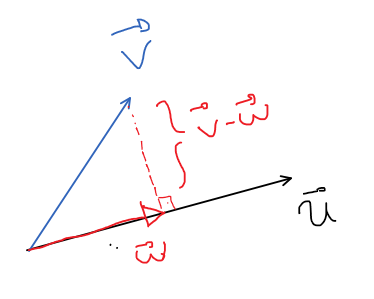
\includegraphics[width=0.4\linewidth]{Imagens/projOrtog}
	\caption{Projeção ortogonal de $v$ em $u$}
	\label{fig:projortog}
\end{figure}

Precisamos de duas premissas, as quais são facilmente observadas na figura acima:
\begin{align*}
	&w=\alpha\cdot u\\
	&\langle u,v-w \rangle=0
\end{align*}
A maneira de encontrar, explicitamente, $w$ em função de $u$ e $v$, com base nessas premissas, está descrita abaixo:
\begin{align*}
	\langle u,v-w \rangle&=0\\
	\langle u,v-\alpha u \rangle&=0\\
	u\cdot v - \alpha\cdot u\cdot u&=0\\
	\alpha\cdot u\cdot u&=u\cdot v\\
	\alpha&=\dfrac{u\cdot v}{u\cdot u}
\end{align*}

Sendo assim, temos:
\begin{equation*}
	w=\left(\dfrac{u\cdot v}{u\cdot u}\right) \cdot u
\end{equation*}

Note que o resultado dos produtos internos entre parênteses é um número, garantindo que $w$ e $u$ são paralelos.

\subsubsection{Matriz de Projeção sobre o vetor $u$}


Podemos encapsular a projeção ortogonal sobre um vetor $u$ em uma matriz $P$, da seguinte forma:
\begin{align*}
	w&=\left(\dfrac{u\cdot v}{u\cdot u}\right) \cdot u\\
	&=\left(\dfrac{u^{T} v}{u^{T} u}\right) \cdot u\\
	&=u\left(\dfrac{u^{T} v}{u^{T} u}\right)\\
	&=\left(\dfrac{u u^{T}}{u^{T} u}\right)v\\
	&=P\cdot v
\end{align*}

\subsubsection{Exemplo:}
Calcule a matriz de projeção sobre o vetor $u=(1,-1,1)$
\begin{align*}
	P&=\left(\dfrac{u u^{T}}{u^{T} u}\right)\\
	P&=\dfrac{1}{3}\begin{pmatrix}
		1 \\
		-1 \\
		1
	\end{pmatrix}\begin{pmatrix}
		1 & -1 & 1
	\end{pmatrix}\\
	P&=\dfrac{1}{3}\begin{pmatrix}
		1 & -1 & 1\\
		-1 & 1 & -1\\ 
		1 & -1 & 1
	\end{pmatrix}
\end{align*}

\subsubsection{Propriedades:}

A matriz $P$ definida possui as seguintes propriedades:
\begin{enumerate}
	\item $P$ é simétrica
	\item $P^2=P$
	\item Posto($P$)=1
\end{enumerate}

\subsection{Projeção Ortogonal sobre um subespaço qualquer}
Considere as matriz $A$ e o vetor $b$ definidos abaixo. Além disso, seja $w$ a projeção ortogonal de $b$ sobre o espaço coluna de $A$.
\begin{equation*}
	A=\begin{pmatrix}
		a_{11} & a_{12} \\
		a_{21} & a_{22}\\
		a_{31} & a_{32} 
	\end{pmatrix},b=\begin{pmatrix}
		b_{11} \\
		b_{21} \\
		b_{31}
	\end{pmatrix}	
\end{equation*}

\begin{figure}[H]
	\centering
	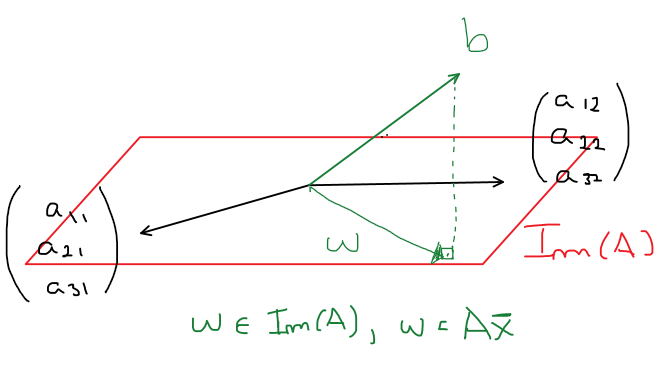
\includegraphics[width=0.4\linewidth]{Imagens/projOrtogEsp}
	\caption{projeção ortogonal sobre imagem de $A$}
	\label{fig:projortogesp}
\end{figure}


Note que:
\begin{enumerate}
	\item o vetor $b-w$ é ortogonal ao espaço coluna de $A$
	\item o vetor $b-A\overline{x}$ é ortogonal ao espaço coluna de $A$, sendo $w=A\overline{x}$.
	\item Logo, $b-A\overline{x}\in $ Núcleo da Transposta de A
	\item $A^T(b-A\overline{x})=0$
	\item $A^Tb=A^TA\overline{x} \rightarrow$ Equação Normal
\end{enumerate}
\textbf{Obs:} se as colunas de $A$ são $LI$, então $A^TA$ é inversível.

Com isso, chegamos na matriz de projeção sobre o espaço coluna de $A$:
\begin{equation*}
	P=A\left(A^TA\right)^{-1}A^T
\end{equation*}
\subsection{Conclusão}
Neste capítulo foram apresentados conceitos projeções ortogonais sobre u vetor e sobre um subespaço vetorial qualquer.

\section{Mínimos Quadrados}

\subsection{Motivação}

Como já sabemos, estamos quase sempre interessados em resolver sistemas do tipo $Ax=b$. No entanto, há casos em que a solução deste sistema é impossível. Por exemplo, se o nosso sistema linear for um sistema linear de equações incompatíveis.

\textbf{Def:} Sistemas lineares incompatíveis são sistemas de $m$ equações e $n$ incógnitas onde $m>n$. Outra maneira de olhar para essa definição é pensar em matrizes $A_{mxn}$, as quais possuem $m$ linhas (equações) e $n$ colunas (incógnitas). Sabemos que sistemas desse tipo não possuem solução.

O que fazer, pode ser feito, além de abandonar o problema e ir dormir em paz, é procurar uma solução aproximada de tal modo que o \textbf{erro} desta solução seja o menor possível. 

\textbf{Def:} o erro de uma solução aproximada de um sistema $Ax=b$, é definido como:
\begin{equation*}
	||Ax-b|| \mbox{ , onde b é a solução real e Ax é a solução aproximada.}
\end{equation*}

Perceba que, para casos em que podemos encontrar a solução real do sistema, esse erro é zero, uma vez que $Ax=b$, logo $||Ax-b||=0$.

Mas e quando não é possível encontrar a solução?

\subsection{Relembrando Projeções Ortogonais}

Lembre-se da capítulo passado sobre projeções ortogonais e acrescente um detalhe.

\begin{figure}[H]
	\centering
	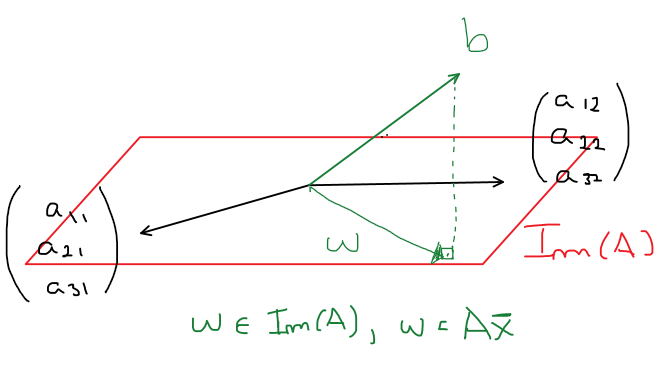
\includegraphics[width=0.4\linewidth]{Imagens/projOrtogEsp}
	\caption{projeção ortogonal sobre imagem de $A$}
	\label{fig:projortogesp}
\end{figure}

No âmbito de minimização de erro, podemos pensar que queremos a menor distância entre a solução real e a aproximada. Sendo assim, a \textit{Projeção Ortogonal} aprendida de mostra muito adequada para esse problema de aproximação.

A própria equação normal $A^TA\overline{x}=A^Tb$ relaciona esses valores. Tenha isso em mente.

\subsection{Mínimos Quadrados}

Uma vez que o sistema linear $Ax=b$ é incompatível, sabemos que $b \notin Col(A)$. Sendo assim, já sabemos que a melhor solução, a que minimiza o erro, será a solução $\overline{x}$ tal que:
\begin{equation*}
	A\overline{x}=Proj_{Col(A)}b
\end{equation*}

Como vimos na aula anterior, podemos definir uma matriz $P$ de projeção sobre o espaço coluna de $A$. Utilizando essa informação, chegamos no seguinte sistema:
\begin{equation*}
	A\overline{x}=Pb
\end{equation*}

Este sistema, agora, é compatível e possui uma solução.

Vejamos, por fim, um exemplo prático de como calcular a melhor reta para um dado conjunto de pontos (regressão linear).

\subsubsection{Exemplo:}
Encontre a reta que melhor interpola os seguintes pontos:
\begin{table}[]
	\centering
	\begin{tabular}{|l|l|}
		\hline
		x  & y \\ \hline
		-1 & 1 \\ \hline
		1  & 1 \\ \hline
		2  & 3 \\ \hline
	\end{tabular}
\end{table}

Dados esses pontos, podemos montar o seguinte sistema linear $Ax=y$:
\begin{equation*}
	\begin{pmatrix}
		1 & x_{1} \\
		1 & x_{2}\\
		1 & x_{3} 
	\end{pmatrix}\cdot 
	\begin{pmatrix}
		b \\
		a 
	\end{pmatrix}=
	\begin{pmatrix}
		y_1 \\
		y_2 \\
		y_3
	\end{pmatrix}
\end{equation*}
\begin{equation*}
	\begin{pmatrix}
		1 & -1 \\
		1 & 1\\
		1 & 2 
	\end{pmatrix}\cdot 
	\begin{pmatrix}
		b \\
		a 
	\end{pmatrix}=
	\begin{pmatrix}
		1 \\
		1 \\
		3
	\end{pmatrix}
\end{equation*}

Rescrevemos como da seguinte maneira:
\begin{align*}
	Ax&=y\\
	A^TAx&=A^Ty
\end{align*}

Colocando valores:
\begin{equation*}
	\begin{pmatrix}
		1 &1 &1\\
		-1 &1& 2
	\end{pmatrix}
	\begin{pmatrix}
		1 & -1 \\
		1 & 1\\
		1 & 2 
	\end{pmatrix}\cdot 
	\begin{pmatrix}
		b \\
		a 
	\end{pmatrix}=
	\begin{pmatrix}
		1 &1 &1\\
		-1 &1& 2
	\end{pmatrix}
	\begin{pmatrix}
		1 \\
		1 \\
		3
	\end{pmatrix}
\end{equation*}

Resolvendo o sistema, encontramos $a=\dfrac{4}{7}$ e $b=\dfrac{9}{7}$.\\

Logo, a reta desejada é: $r(x)=\dfrac{4}{7}\cdot x + \dfrac{9}{7}$

\subsection{Conclusão}
Neste capítulo foi relembrado o conceito de projeções ortogonais sobre um subespaço vetorial qualquer e apresentado o algoritmo de Mínimos Quadrados.


\section{Matrizes Ortogonais, Ortogonalização de Grand-Schimdt e Fatoração QR}

\subsection{Matrizes Ortogonais}

Para definir uma matriz ortogonal, precisamos lembrar o que é um conjunto de vetores, ou uma base, se quisermos, ortonormal.\\

\textbf{Def:} uma base $\beta$ de vetores de $R^n$ é dita ortonormal se todos os vetores que a formam possuem, simultaneamente, norma 1 e são ortogonais entre si.\\

Com essa definição, podemos definir tranquilamente uma Matriz Ortogonal.\\

\textbf{Def:} Uma Matriz Ortogonal $A$ é uma matriz cujas colunas formam uma base ortonormal. \\

Algumas propriedades das matrizes ortogonais são importantes para nosso curso.

\subsubsection{Propriedades}

\textbf{(1)} Toda matriz ortogonal $Q$ satisfaz $Q^{T}Q=I$. Dessa propriedade, nota-se que $Q^T=Q^{-1}$\\

\textit{Prova:} note que uma multiplicação matricial é, de certo modo, um produto interno entre as colunas e linhas das matrizes. Sendo assim, como as colunas de $Q$ são ortonormais, $\langle v_i,v^{T}_{j} \rangle=0 \forall i\neq j$, sendo $v_i$ os vetores da coluna de $Q$ e $v_j$ os vetores linhas de $Q^T$. A partir disso mostramos que $Q^TQ=I$.  \\

\textbf{(2)} A multiplicação de uma matriz ortogonal por um vetor preserva o comprimento do vetor $\rightarrow ||Qx||=||x||$. \\

\textit{Dem:} $||Qx||^2 = \langle Qx,Qx \rangle=(Qx)^TQx=x^TQ^TQx=x^Tx=||x||^2$\\

\textbf{(3))} O ângulo entre vetores se preserva por matriz ortogonal.\\

\textit{Dem:} $cos\theta=\dfrac{\langle Qu,Qv \rangle}{||Qu|||Qv|||}=\dfrac{uQ^TQv}{||u|||v|||}=\dfrac{u^Tv}{||u|||v|||}$

\subsection{Ortogonalização de Grand Schimdt}

O processo de ortogonalização de Grand-Schimdt consiste em uma estratégia para, a partir de uma base qualquer $\{a_1,...,a_n\}$, obter uma base ortonormal $\{q_1,...q^n\}$ para o espaço gerado pela base $a$. Temos a seguinte construção:
\begin{align*}
	&a_1^{'}=a_1 \rightarrow q_1=\dfrac{a_1^{'}}{||a_1^{'}||}\\
	&a_2^{'}=a2-(q_1^Ta_2)q_1 \rightarrow q_2=\dfrac{a_2^{'}}{||a_2^{'}||}\\
	&a_3^{'}=a3-(q_1^Ta_3)q_1 -(q_2^Ta_3)q_2\rightarrow q_3=\dfrac{a_3^{'}}{||a_3^{'}||}\\
	&a_n^{'}=an-(q_1^Ta_n)q_1 -...-(q_{n-1}^Ta_n)q_{n-1}\rightarrow q_n=\dfrac{a_n^{'}}{||a_n^{'}||}
\end{align*}


\subsection{Fatoração QR}

O processo de ortogonalização de Grand Schimdt nos entrega uma fatoração conhecida como \textbf{fatoração $A=QR$}. Não é difícil imaginar que a matriz $Q$ desta fatoração será a matriz cujas colunas são a base $\{q_1,...q^n\}$ obtida no processo de ortogonalização e $A$ é a matriz cujas colunas são a base $\{a_1,...,a_n\}$.\\

Antes de definirmos a matriz $R$, lembremos:\\	

Se $\{q_1,...q^n\}$ é base ortonormal de $R^N$ e $b$ pertence a esse espaço gerado, então...
\begin{equation*}
	b=c_1q_1+c_2+q_2+...+c_nq_n
\end{equation*}
onde
\begin{equation*}
	c_1=q_1^Tb, c_2=q_2^Tb... c_n=q_n^Tb
\end{equation*} 

Vejamos como construir a matriz $R$ para o caso de uma base do $R^3$. Esse procedimento é facilmente generalizado para $R^N$.

\textbf{Exemplo:} Seja $\{a,b,c\}$ base para o $R^3$ e $\{q_1,q_2,q^3\}$ base ortonormal obtida via ortogonalização de Grand Schimdt a partir da base $\{a,b,c\}$.\\

Temos que:\\

$a=(q_1^Ta)q_1+(q_2^Ta)q_2+(q_3^Ta)q_3=(q_1^Ta)q_1$\\

A primeira coluna de $R$ será, então, $(q_1^{T}a,0,0)^T$\\

$b=(q_1^Tb)q_1+(q_2^Tb)q_2+(q_3^Tb)q_3=(q_1^Tb)q_1+(q_2^Tb)q_2$\\

A segunda coluna de $R$ será, então, $(q_1^{T}a,q_2^Tb,0)^T$\\

$a=(q_1^Tc)q_1+(q_2^Tc)q_2+(q_3^Tc)q_3$\\

A terceira coluna de $R$ será, então, $(q_1^{T}a,q_2^Tb,q_3^Tc)^T$\\

Logo, $R=\begin{pmatrix}
	q_1^{T}a & q_1^{T}a & q_1^{T}a\\
	0 &  q_2^Tb& ,q_2^Tb\\ 
	0 & 0 & q_3^Tc
\end{pmatrix}$

\subsection{Conclusão}
Neste capítulo apresentados os conceitos de Matriz Ortogonal, Processo de Ortogonalização de Grand-Schimdt e Fatoração $A=QR$.
\end{document}

